% 76-29(76쪽) — $-\pi<x<3\pi$ 에서 $y=\tan\dfrac{1}{2}x$ 의 그래프와 두 직선 $y=2k$, $y=-k$ 로 둘러싸인 도형(원문 「오른쪽 그림」).
% 스캔 화질이 낮아 TikZ 로 다시 그림. 라벨은 원문 것만: $x$축의 $-\pi$·$\pt{O}$·$\pi$·$2\pi$·$3\pi$, 두 직선 이름, 곡선 이름.
% $x$ 한 칸은 $\pi$. $y$ 눈금은 원문에 없으므로 적지 않는다 — 넓이 $18\pi$ 에서 구하는 $k$(답)가 그림에서 읽히지 않게 한다.
\begin{tikzpicture}[line width=0.6pt, x=0.78cm, y=0.50cm, >=stealth]
  \fill[black!10]
    plot[domain=-0.5:0.7048, samples=70, smooth] (\x, {tan(90*\x)}) --
    plot[domain=2.7048:1.5, samples=70, smooth] (\x, {tan(90*\x)}) -- cycle;
  \draw[densely dotted, line width=0.45pt] (-1,-2.9) -- (-1,2.9);
  \draw[densely dotted, line width=0.45pt] (1,-2.9) -- (1,2.9);
  \draw[densely dotted, line width=0.45pt] (3,-2.9) -- (3,2.9);
  \draw[line width=0.55pt] (-1.4,2) -- (4.9,2);
  \draw[line width=0.55pt] (-1.4,-1) -- (4.9,-1);
  \draw[->, line width=0.7pt] (-1.5,0) -- (5.05,0);
  \draw[->, line width=0.7pt] (0,-3.1) -- (0,3.1) node[left=1pt, font=\small] {$y$};
  \draw[domain=-0.787:0.787, samples=110, smooth] plot (\x, {tan(90*\x)});
  \draw[domain=1.213:2.787, samples=110, smooth] plot (\x, {tan(90*\x)});
  \node[font=\small, anchor=south west] at (3.50,2.12) {$y=2k$};
  \node[font=\small, anchor=north west] at (3.50,-1.12) {$y=-k$};
  \node[font=\small, anchor=south east] at (5.00,0.08) {$x$};
  \node[font=\small, fill=white, inner sep=1pt, anchor=north] at (-1,-0.10) {$-\pi$};
  \node[font=\small, anchor=north west] at (0.05,-0.10) {$\pt{O}$};
  \node[font=\small, fill=white, inner sep=1pt, anchor=north west] at (1.02,-0.10) {$\pi$};
  \node[font=\small, anchor=north] at (2,-0.10) {$2\pi$};
  \node[font=\small, fill=white, inner sep=1pt, anchor=north] at (3,-0.10) {$3\pi$};
  \node[font=\small, anchor=north] at (1.75,-3.05) {$y=\tan\dfrac{1}{2}x$};
\end{tikzpicture}
